% !TeX spellcheck = en_US
\section{Experimental Design}\label{sec:experimental_design}

In this section, we present the image datasets used for the training, validation and test steps, we expose the details of our implementation of both \glspl{cnn}, we show how the images are pre-processed before the training and we described the followed training strategies and set of experiments.

\subsection{Training, Validation and Test datasets}

For training and validation, BSD200 \cite{BSDS}, General100 \cite{FSRCNN} and T91 \cite{T91} datasets have been used, bringing the total of images to 391. A 10\% of these images have been randomly chosen for validation, therefore, the training set has 352 images and the validation set, 39.

Set5 \cite{SET5} and Set14 \cite{SET14} have been used for the test stage, making a total of 19 images.

The same training, validation and test datasets have been used for both \gls{fsrcnn} and \gls{ircnn}. 

\subsection{Implemented \glspl{cnn}}
For this study, we have used our own implementation of \gls{fsrcnn} and \gls{ircnn} using Keras \cite{KERAS} in order to use the same deep learning framework for both networks.

Both of them use a sequential model in order to stack bi-dimensional convolution (or deconvolution) layers. All the layers use the format \gls{nhwc}.

In order to deal with the boundary artifacts produced by the convolution operation, zero padding has been adopted in all layers according to the filter size.

For FSRCNN, the filters are initialized with variance scaling for all the convolution layers and with a Gaussian distribution with zero mean and standard deviation 0.001 for the deconvolution layer. Furthermore, for the mapping depth, the LR feature dimension and the number of shrinking filters, we have used, $m=4$, $d=48$ and $s=16$, respectively, since in \cite{FSRCNN}, these settings show outstanding \gls{psnr} results compared to the rest of investigated settings.

For IRCNN, glorot uniform initializer \cite{XAVIER} is used to initialize the filters of all the convolution layers.

All the implementation details of the \glspl{cnn} and the datasets used can be found at \href{https://github.com/guillermoruizalv/restore}{https://github.com/\\guillermoruizalv/restore}.

\subsection{Image pre-processing}
Before being used as input of the neural networks, the 391 images used for training and validation are pre-processed using some common and some model-dependent steps:
\begin{itemize}
	\item First, since we are using \gls{rgb} images with true color (24 bits, 8-bits per channel), all the images are loaded as 3-dimensional matrices using uint8 (unsigned 8-bit integer) data type.
	
	Only for \gls{fsrcnn}, the images are converted from \gls{rgb} to \gls{ycbcr}. Specifically, the $Y$ component is super-resolved by the network and the blue-difference and red-difference components are upscaled using bicubic interpolation.
	
	\item Once the images are loaded, they are scaled to $[0,1]$ range and transformed to float64 (double precision floating-point format). 
	
	\item The resulting images are cropped into $32\times32$ sub-patches using a stride of size $16$ in order not to lose the information between adjacent patches. The remaining pixels are discarded.
\end{itemize}

This process results in 170293 sub-patches for training and 20705 sub-patches for validation.

A last pre-processing step is applied to the training and validation images depending on the model that is going to be trained.
\begin{itemize}
	\item For \gls{fsrcnn}, Lanczos interpolation is used in order to downscale the data using a scale factor of 2. Before downscaling, if the number of rows or the number of columns is not even, the bottom-most row or the right-most column are discarded, respectively. This is done so that when \gls{fsrcnn} upscales the image, the output of the network has the same dimensions as the labels.
	\item For \gls{ircnn}, random noise is added to the patches using the following parameters:
	\begin{itemize}
		\item The noise method to be applied is chosen randomly from Gaussian noise, Poisson noise, salt-and-pepper noise and uniform noise using the same probability.
		\item If Gaussian noise is selected, $\mu$ is set to 0 and $\sigma$ takes a random value from the range $[0.05, 0.15]$.
		\item If Poisson noise is selected, input pixel values are interpreted as means of Poisson distributions scaled up by $2^8$.
		\item If salt-and-pepper noise or uniform noise is selected, the noise ratio takes a random value from the range $[0.05, 0.20]$.
	\end{itemize}
\end{itemize}

\subsection{Training hardware, strategy and results}
\paragraph{Training hardware}
The training has been carried out in a server running Ubuntu 18.04 LTS with a Nvidia Geforce GTX 1060 with compute capability of $6.1$. Most of the development has been done in a different machine with the same \gls{os} and a Nvidia Geforce GT 730M with compute capability of $3.5$.

\paragraph{Training strategy}
The training strategy adopted for \gls{fsrcnn} and \gls{ircnn} is common for both cases except for the used learning rates.

\begin{itemize}
	\item \textbf{Image loading and memory management}. Due to the big amount of data used for the training, the training and validation images have been loaded dynamically so that the pre-processing held a maximum of 64 images at a time. 
	
	This allowed us to consume less memory resources on both the machine and the \gls{gpu} that have been used for the experiments, given their memory limitations. Consequently, the training performance was slightly reduced since for each epoch, the training images had to be loaded multiple times.
	
	\item \textbf{Batch size}. A batch size of $256$ samples has been selected, producing $666$ batches for the training images and $81$ batches for the validation images.
	
	\item \textbf{Reproducibility and number of threads}. In order to be able to reproduce the noise generation, we set the random seed of the \textit{numpy.random} module to $1$ at the beginning of each epoch. 
	
	However, unlike the \textit{random} module, \textit{numpy.random} is not thread-safe. For this reason, we have set the number of threads to $1$ slightly losing some performance when generating the training images but having the ability to generate equal noisy sub-patches for each epoch.
	
	\item \textbf{Loss function}. The loss function used in both cases is \gls{mse}:
	$$MSE = \frac{1}{n}\sum_{i=0}^{n}\left(Y_{pred}-Y_{true}\right)$$
	where $Y_{pred}$ is the predicted result of the network and $Y_{true}$ is the value of the label.
	\item \textbf{Optimizer}. The Adam optimizer \cite{ADAM} has been used for both models. Although \gls{sgd} is proposed in \cite{FSRCNN} for training \gls{fsrcnn}, we empirically found that the Adam optimizer offered better training performance.
	
	The selected learning rates for this optimizer are:
	\begin{itemize}
		\item For \gls{fsrcnn}, an initial learning rate of $10^{-3}$ is used. This value is reduced to a minimum of $10^{-4}$ using a patience of $10$ on the validation set. This means that the learning rate is reduced when the validation loss has stopped improving for $10$ epochs in a row.
		\item For \gls{ircnn}, an initial learning rate of $10^{-4}$ is used. For this model, the patience is also set to $10$, after which the learning rate is reduced to a minimum of $10^{-5}$. 
		
		Our initial experiments with \gls{ircnn} were using the same learning rate values as \gls{fsrcnn}. However, we noticed that the model stopped learning very early and that the loss function on the training and validation datasets was oscillating over the training epochs. For this reason, the learning rate values were reduced with a scale of $0.1$, improving the training performance.
	\end{itemize}
    \item \textbf{Early stopping}. Instead of setting a specific number of training epochs, we monitor the performance of the models and we use early stopping on the validation loss with a patience of $25$. This means that if the validation loss has not improved after 25 epochs in a row, the training will be automatically stopped.
    
    The reason why we use early stopping instead of a given number of epochs is to avoid over-training,   reduce over-fitting and improve the generalization of the \glspl{cnn}.

\end{itemize}

\paragraph{Training results}
Using this training strategy, we have had the following training results:
\begin{itemize}
	\item \gls{fsrcnn} was trained for 1092 epochs during approximately one day, reaching a minimum validation loss value of $0.0011$.
	\item \gls{ircnn} was trained for 891 epochs during approximately four days, reaching a minimum validation loss value of $5.0165\times10^{-4}$.
\end{itemize}

The learning curves of both \glspl{cnn} are presented in Figure \ref{fig:training}. We can observe that, for \gls{ircnn}, the validation loss is oscillating around epoch $50$. After $10$ epochs, the learning rate is reduced with a scale factor of $0.1$ and the validation loss continues decreasing.

In earlier experiments, the training was stopping at this stage after 25 epochs before we reduced the learning rate to a minimum of $10^{-5}$.

\begin{figure}[h]
	\centering
	\begin{subfigure}{0.49\textwidth}
		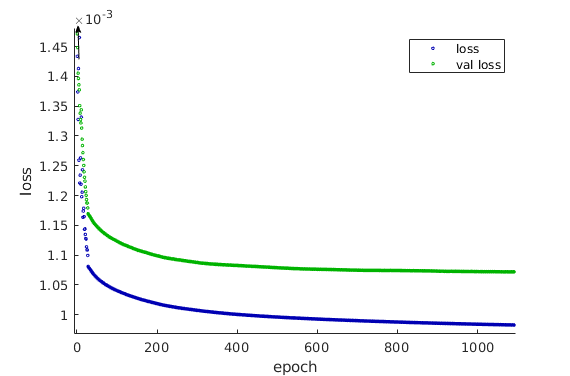
\includegraphics[width=\textwidth]{images/fsrcnn_train.png}
		\caption{\gls{fsrcnn}}
	\end{subfigure}
	\begin{subfigure}{0.49\textwidth}
		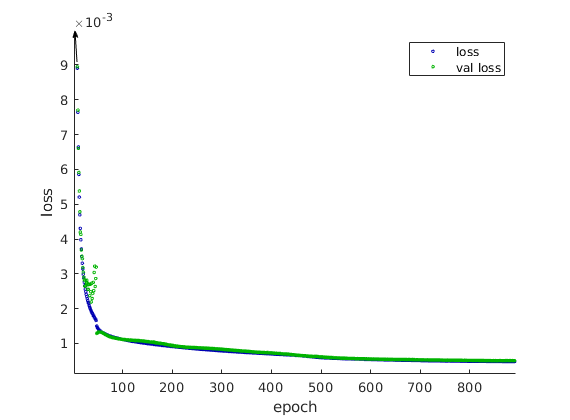
\includegraphics[width=\textwidth]{images/ircnn_train.png}
		\caption{\gls{ircnn}}
	\end{subfigure}
	\caption{\glspl{cnn} learning curves.}
	\label{fig:training}
\end{figure}

\subsection{Set of experiments}
We have carried out the following set of experiments using Set5 \cite{SET5} and Set14 \cite{SET14} as test datasets:
\begin{itemize}
	\item \textbf{Experiment 1.1}: Evaluation of \gls{fsrcnn} $+$ \gls{ircnn} on Set5 and Set14.
	\item \textbf{Experiment 1.2}: Evaluation of \gls{ircnn} $+$ \gls{fsrcnn} on Set5 and Set14.
\end{itemize}

The aim of these two experiments is to get to know which combination performs better on the given noisy images.

Apart from these and given their results, we also perform the following experiments in order to evaluate the performance of the deep learning methods compared to the selected traditional methods. This set of experiments use a deep learning method and a traditional method for either \gls{sisr} or image denoising:
\begin{itemize}
	\item \textbf{Experiment 2.1}: Evaluation of \gls{ircnn} $+$ bicubic interpolation.
	\item \textbf{Experiment 2.2}: Evaluation of wavelet denoiser $+$ \gls{fsrcnn}.
	\item \textbf{Experiment 2.3}: Evaluation of median filter $+$ \gls{fsrcnn}.
\end{itemize}

Finally, the following set of experiments is carried out to have a benchmark based purely on traditional algorithms:
\begin{itemize}
\item \textbf{Experiment 3.1}:  Evaluation of wavelet denoiser $+$ bicubic interpolation.
\item \textbf{Experiment 3.2}:  Evaluation of median filter $+$ bicubic interpolation.
\end{itemize}
All these experiments are carried out using \gls{psnr} and \gls{ssim} as quality metrics.